\documentclass[11pt]{report}
\pagestyle{plain}
\usepackage{graphicx}
\usepackage{indentfirst}
\usepackage{float}
\usepackage[top=2.5cm, left=2.0cm, right=2.0cm, bottom=2.5cm]{geometry}
\newcommand{\unit}[1]{\ensuremath{\, \mathrm{#1}}}
%\restylefloat{table}
%\restylefloat{figure}
\usepackage{amssymb}
\usepackage{amsmath}
\usepackage{amsfonts}

\newcommand{\horline}{\begin{center} \line(1,0){470} \end{center}}


\author{Francisco Machado}
\title{SED fitting Project}
\begin{document}

\maketitle

{\bf What is the project?}

The project I am developing is a tool that will allow the use of the galaxies from the Illustris simulation to gain a better estimate of the properties of real galaxies.

By comparing the SED of the simulation galaxies and the observed galaxies we can infer the properties of the galaxy.\\

{\bf What is the normal procedure so far?}

The current way of estimating the masses of the galaxies is by creating a set of artificial SED's based on a certain set of properties (this method is called Synthetic Stellar Population (SSP)). The problem with this method is two fold, first is that the galaxies are created from a set of values for each property that has a very discrete nature, meaning that for each property there are a discrete set of values and you then create an SED for each combination of properties.

The second problem is that the models used for the construction of these SED is very limited. In the GAMA survey they assumed a constant metalicity, a constant dust absorption and an exponential stellar formation rate. Assumptions which limit which put constrains in the synthetic SED, which may not happen in the SED's we want to fit.\\

{\bf How am I doing it?}

Two ideas have been developed, one which corresponds to a best fit and another where the properties are calculated using Baysean statistics.

On the first one, the idea is to compare the input galaxy with all the Illustris Galaxies using the $\chi^2$ test. From there we can choose the one galaxy in the simulation with the lowest value and attribute the properties of that galaxy to our input galaxy.

This has the pitfall that if the input galaxy is close to many galaxies, only one is considered and the information about the others is discarded. Nevertheless we obtained close, but not perfect values for the fitting and the masses:

Example:
\begin{figure}[H]
\centering
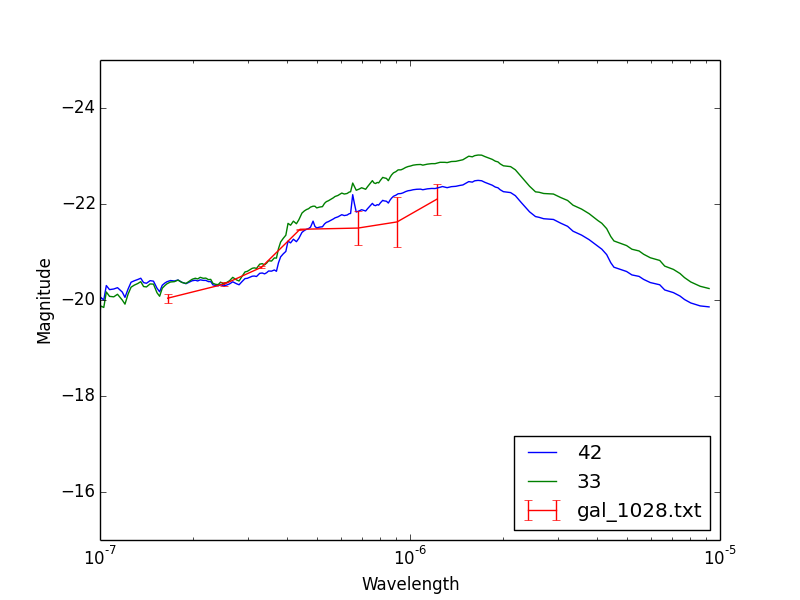
\includegraphics[width = 0.8\textwidth]{Graphs/42_33_gal_1028.png}
\caption{Example of a fit done by the best fit comparison. gal\_1028 is the galaxy SED we are trying to fit while 42 and 33 are the best two fits from the Illustris SED}
\end{figure}

Plotting a comparison between the masses obtained by the best fit and the masses that the GAMA survey presents gives us:
\begin{figure}[H]
\centering
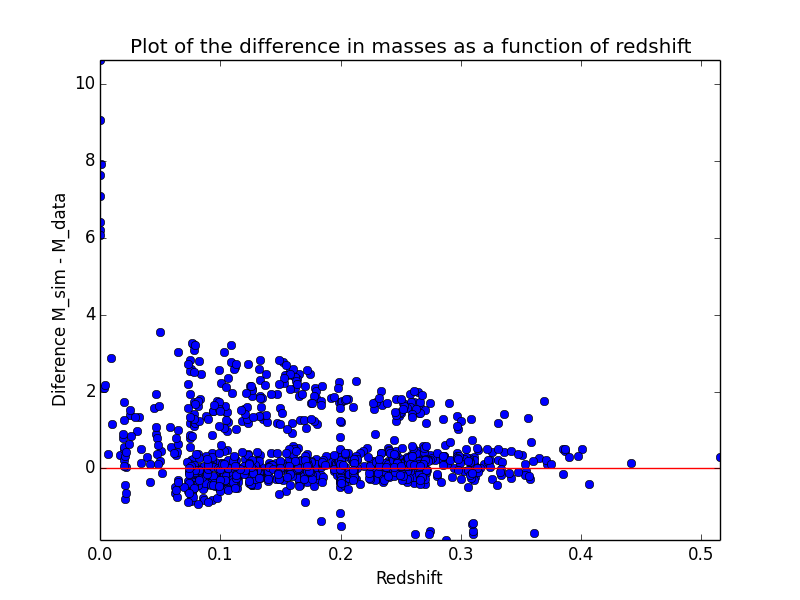
\includegraphics[width = 0.8\textwidth]{Fits_Galax/red_dif.png}
\caption{Difference between the estimated masses and the data masses.}
\end{figure}

The other alternative is to make use of Baysean statistics to calculate the properties of the galaxy.

The idea is to do a weighted average on the property of the galaxy of interest, such that each weight is the probability of given a our input galaxy that that galaxy is a the correct description $P(S|I)$.

Using Bays Theorem we have $P(S|I) = P(I|S) \times P(S)$. (The probability of our input galaxy is one).

But $P(I|S)$ is given by the $\chi^2$  in the form $e^{-\chi^2}$. $P(S)$ is another factor which is gives the probability of that simulated existing. For now we set this to be equal for all, but it could be a parameter worth exploring.

Since the Baysean approach takes into account all the galaxies at once, in principle it will provide better estimates, but right now the goal is to evaluate the difference between the two methods and between the methods and the properties reported.

To do this comparison I am using the GAMA survey data which contains SEDs and the value of many properties of the galaxies.\\

Ploting the same graph for the Baysean we have:

\begin{figure}[H]
\centering
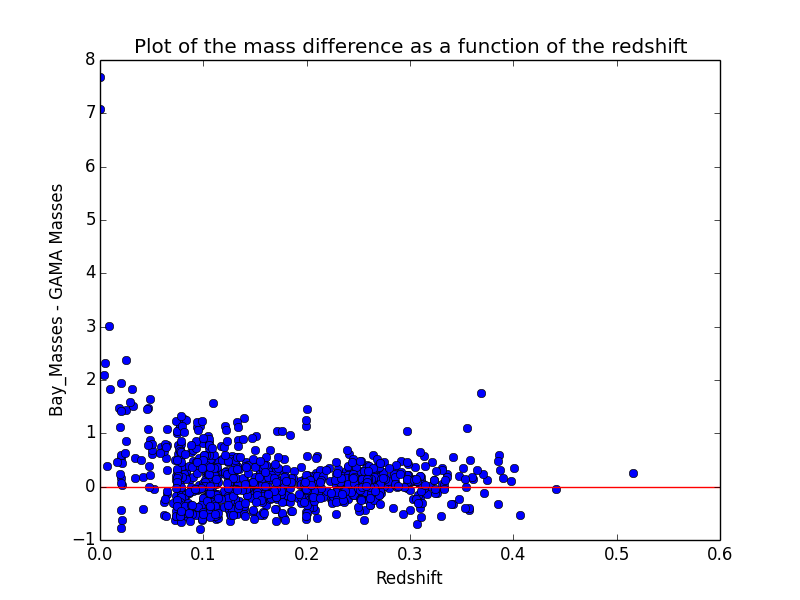
\includegraphics[width = 0.8\textwidth]{Results_Bay/diff_red.png}
\caption{Difference between the estimated masses and the data masses.}
\end{figure}

Then other plots can be made:

\begin{figure}[H]
\centering
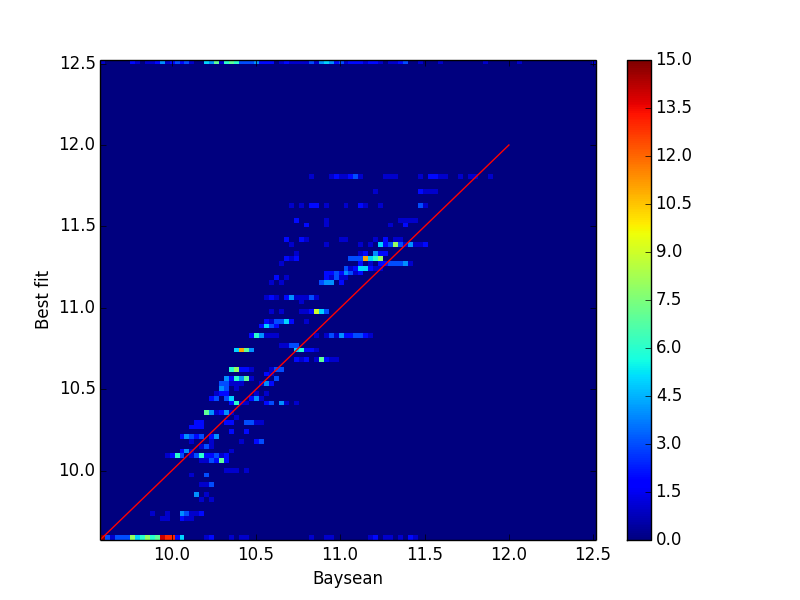
\includegraphics[width = 0.8\textwidth]{Results_Bay/Bay-Best.png}
\caption{Difference between the masses of the two methods.}
\end{figure}




{\bf Where to go next?}

Besides an more exaustive analysis on the distributions of the calculations for the various methods, it will be important to optimize the code.

Right now, in my computer, using half of Illustris I am getting about 20min per galaxy compared, so this data was compiled with a subset of the Illustris data, only 100 SED.\\

Another idea to speed up the calculations was to make use of machine learning algorithms, in particular algorithms of clustering/categorizing. By finding classes of galazies within Illustris we could then select a representative of each galaxy and compare with those, before comparing with the entire class. Since the $\chi^2$ is on an exponential this method could provide good calculated values, however it would be necessary to check and see if this prediction is true.

Another idea we had was to try to find patterns on the data we have. Again using machine learning algorithms to see if we can relate features in the SED to properties of the system, and if so, why is that so.
\end{document}

